\justifying
\NSFCBodyText

\subsubsection{研究内容}
\textbf{内容一：未见矿区变化检测的误差诊断。}
以MineNetCD为主数据，核对矿区、原始影像与切片的来源关系，复现官方划分下的代表性基线，按矿区分析误报与漏检。抽查高置信度误检、漏检和随机正常样本，区分配准差异、标签边界、背景外观差异与真实细小变化。建立可追溯的误差清单，判断一致性约束是否确为值得研究的主要因素。该内容为机制实验提供分层标准和比较对象，矿区划分本身沿用已有原则。

\textbf{内容二：跨时相一致性约束的作用区域与负迁移条件。}
在同一骨干上改变约束所覆盖的区域，检验全图一致性、标注未变化区一致性与等面积随机约束对误报、细小变化召回的不同影响。在固定约束面积下调节其中变化像素的比例，观察特征距离、监督梯度与检测错误的共同变化，排除约束强度、边界筛选和平滑造成的替代解释。完整FCCDN、DonaNet及可复现的CDDGNet作为独立方法比较，不以简化消融替代其原方法。最终形成约束适用条件和反例，而非只给出一个总体增益。

\textbf{内容三：固定复核面积下的可靠性评价。}
对冻结检测器开展独立矿区校准，构建由概率熵与固定多视图推理分歧组成的简单错误排序。将整幅有效区域划为窗口，比较同一面积预算下剩余误报与漏检，检查高置信度未变化预测中的错误。先评价理想纠错模拟的上限，再在合作者落实后开展小规模真实复核，分别记录面积、窗口数与工时。EuroMineNet作为条件性扩展，优先验证方法在其内部未见矿区的适用性。

三项研究依次提供误差证据、约束效应和复核评价，总体关系见图\ref{fig:mct-framework}。
\begin{figure}[!htbp]
  \centering
  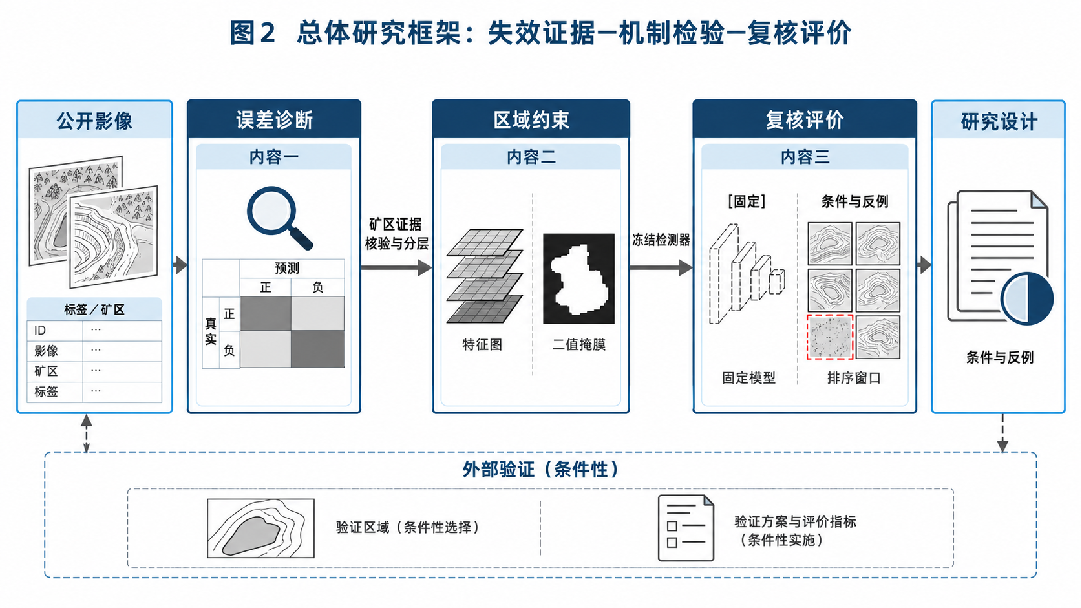
\includegraphics[width=\linewidth,trim=0 0 0 12mm,clip]{figures/F02_overall_framework.pdf}
  \captionsetup{justification=justified,singlelinecheck=false}
  \caption{总体研究框架。误差诊断向区域约束实验提供核验样本和分层规则；检测器冻结后开展复核评价，汇总适用条件与反例。外部验证为核心实验完成后的条件性扩展。}
  \label{fig:mct-framework}
\end{figure}

\subsubsection{研究目标}
总体目标是在公开矿山数据上解释一致性约束对变化判别的条件性作用，并检验预测可靠性信息能否帮助识别未见矿区的错误。

一是建立可重复运行的矿区级误差诊断与对照协议，明确影响结论的数据条件。二是检验背景限定约束相对于同骨干全图约束的误报改善与细小变化召回非劣关系，识别其成立或失效的范围。三是量化错误排序相对随机和单指标基线的复核收益与代价，形成全图剩余错误及变化覆盖的评价结果。目标以效应量、区间和对照证据衡量，不在无前测条件下承诺任意精度涨幅。

\subsubsection{拟解决的关键科学问题}
\textbf{问题一：约束区域如何影响变化敏感性？}
未变化地物的两期特征差异可能包含观测干扰，真实变化的特征差异则承载判别信息。同一一致性目标在两类区域中可能产生不同作用。本项目通过固定面积的约束污染与自然矿区分层，检验这种作用是否依赖变化比例、变化尺度及外观差异，而不是仅由总体正则强度决定。

\textbf{问题二：概率与推理稳定性能够识别哪些预测错误？}
校准概率接近经验正确率，并不保证能发现所有高置信度漏检。拟比较概率熵和多视图分歧的互补范围，判断组合排序是否在低复核预算下仍有增量，及其是否把收益集中到容易发现的误报而遗漏真实变化。

\textbf{问题三：这些关系在何种矿区和观测条件下能够重现？}
以矿区为独立评估单位，分析不同外观差异和变化尺度下的效应及反例。对跨数据集结果先解决输入与标签口径，再解释可重复性，防止把观测系统差异误写成算法泛化机制。

\subsubsection{研究方法与技术路线}
研究按“数据与来源核验—基线误差诊断—约束区域对照—可靠性评价—矿区级统计与反例解释”推进。首阶段输出数据清单、固定划分及基线误差证据；只有确认主要误差与拟研究机制相关，才进入背景限定约束实验。之后冻结检测器，独立评价校准与复核排序，避免两个模块同时变化造成归因不清。最后整合不同矿区、干扰分层和变化尺度下的证据，形成适用范围与失败案例。

\textbf{对应内容一的数据与误差路线（图\ref{fig:mct-route-diagnosis}）。}输入公开影像、标签和矿区元信息，经过来源审计、基线复现及分层抽查，输出固定划分与可追溯误差清单。以配对完整性、矿区隔离和误差核验一致性检查质量，确定内容二使用的样本范围及干扰分层。

\textbf{对应内容二的区域约束路线（图\ref{fig:mct-route-constraint}）。}输入经核验的数据、基线和分层规则，开展同骨干区域对照、强度匹配和近邻掩码替换，输出效应区间、适用条件与失败案例。以误报和小变化召回联合评价收益，以随机和平滑对照检查替代解释；检测器配置在开发集确定后冻结，供内容三评价其可靠性。

\textbf{对应内容三的复核评价路线（图\ref{fig:mct-route-reliability}）。}输入冻结检测器、独立校准矿区及预列评分规则，经温度拟合、验证集规则选择和全图窗口排序，输出固定面积预算下的剩余错误与覆盖曲线。用相同检测器上的随机及单指标对照验证增量，再结合内容一的误差类型解释排序盲区，汇入最终矿区级证据报告。

首阶段若发现主要问题为配准或标签歧义，则先开展相应质量诊断，并据结果调整假说。核心方法无增量时，保留严格对照与负结果，停止叠加额外网络模块。外部数据与真实人员复核均设在核心实验之后，不影响主数据上的最小研究闭环。

围绕上述路线，分别开展主检验、辅助检验和条件探索，具体比较与判据如下。
\begin{center}
\begin{tabular}{p{0.14\linewidth}p{0.28\linewidth}p{0.39\linewidth}}
\hline
任务 & 首要比较 & 支持条件与解释范围 \\
\hline
主检验 & 同骨干背景约束对全图约束 & 误报改善且小变化召回非劣；随机、强度及平滑对照用于排除替代解释。 \\
辅助检验 & 固定检测器的组合排序对最强单指标 & 同预算及同实际面积核对下，剩余误报与漏检均改善；仅解释离线纠错上限。 \\
条件探索 & 外观分层、掩码污染及近邻局部替换 & 报告效应差和反例，不以总体收益、单层显著或梯度现象单独证明机制。 \\
\hline
\end{tabular}
\end{center}
\textbf{（1）数据验收与独立划分。}
先下载并校验MineNetCD正式归档，登记版本、许可证、文件校验值、矿区ID及场景来源；检查影像与标签配对、有效像素和配准质量。重复或无效样本按事先固定的规则处理，保留剔除原因；不得依据模型测试表现删除困难矿区。原论文60/10/30矿区划分用于官方协议复现。为分离校准与选择，主机制实验采用\textbf{【暂定 50个训练矿区、10个独立校准矿区、原10个验证矿区与原30个测试矿区；名单在归档核验后冻结】}。校准矿区从原训练部分划出，所有主比较方法在相同训练矿区重新训练。

前期误差诊断和规则设计只使用训练及验证矿区，校准矿区仅承担温度拟合。首先在主协议训练与验证部分复现官方方法配置；官方60/10/30完整协议的训练与测试复现推迟至主协议全部冻结后，结果单列。

训练集用于拟合模型，验证集用于选择方法、阈值和复核规则，校准集只拟合温度参数，测试集用于冻结后的评估。先在开发矿区选定检测器配置，随后每个随机种子仅在校准集拟合一次温度；验证集只从预列的评分候选中选择规则，不随验证反馈重拟温度。测试标签在全部规则锁定前不参与任何决策。归一化统计、增强选择和预训练权重的矿区覆盖均纳入审计。官方权重复现与主协议重训单列，避免把60矿区训练的结果直接与50矿区结果比较。无标签适应、少样本微调若开展，另外记录可见信息范围。

\begin{figure}[!htbp]
  \centering
  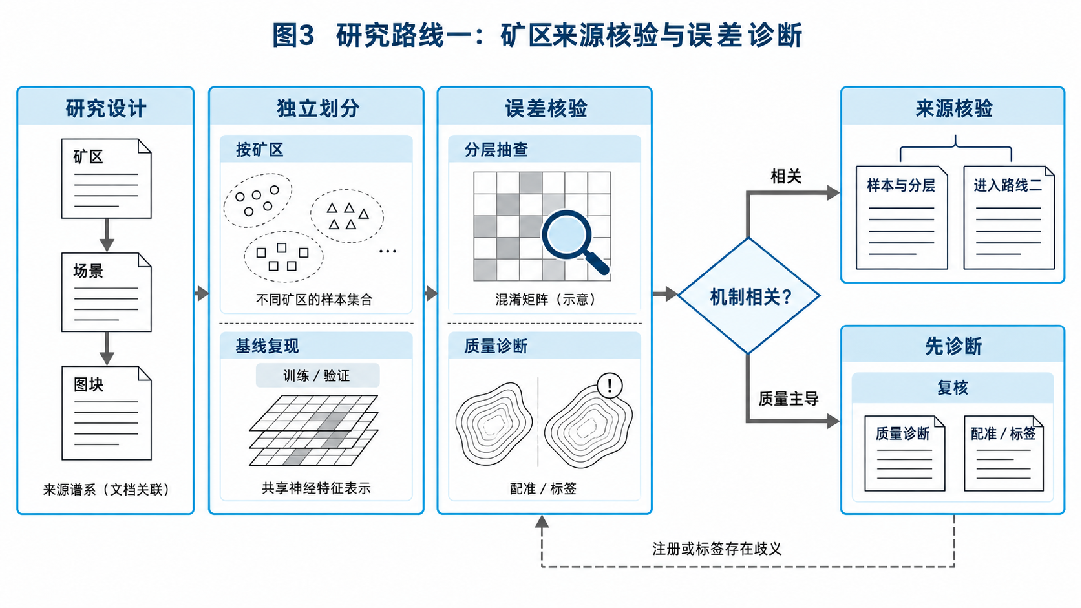
\includegraphics[width=\linewidth,trim=0 0 0 12mm,clip]{figures/F03_route_diagnosis.pdf}
  \captionsetup{justification=justified,singlelinecheck=false}
  \caption{研究路线一：矿区来源核验与误差诊断。开发期依次核对矿区、场景和切片来源，复现基线并抽查误差；配准或标签歧义主导时先返回质量诊断，再确定进入机制实验的样本与分层。}
  \label{fig:mct-route-diagnosis}
\end{figure}
\FloatBarrier

\textbf{（2）背景限定约束与可归因对照。}
给定两期影像$x^{(1)},x^{(2)}$及训练变化标签$Y$，以$Y=0$的有效区域经边界腐蚀形成掩码$M$，称为标注未变化区。令$f^{(t)}_i$为共享编码器在位置$i$的特征，$\bar f^{(t)}_i$为其单位化形式，构建
\begin{equation}
\mathcal{L}_{\mathrm{bg}}=\frac{\sum_i M_i\|\bar f_i^{(1)}-\bar f_i^{(2)}\|_2^2}{\max(1,\sum_i M_i)},\qquad
\mathcal{L}=\mathcal{L}_{\mathrm{seg}}+\lambda\mathcal{L}_{\mathrm{bg}}.
\end{equation}
分割监督$\mathcal{L}_{\mathrm{seg}}$覆盖全部有效变化与未变化像素。空掩码时背景约束为零；特征单位化采用小正数防止零范数。训练掩码只由训练标签产生，测试前向不使用真值选择背景。腐蚀尺度与约束强度在验证集上按同等搜索预算选择。

受控实验包括无一致性、全图一致性、背景限定一致性和等面积随机一致性四组。全图组约束全部有效区域，随机组的像素数与背景组一致；各损失均按实际约束像素数归一化。随机掩码进一步匹配空间形状与边界距离分布，记录无法匹配的样本比例及变化像素覆盖，避免把样本筛选效应归于“背景稳定”。在同一分割结果上增加同等调参预算的平滑对照，检查误报下降是否以边界或细小目标损失为代价。模型容量、训练步数、输入分辨率和增强策略保持一致，并记录梯度范数，补充总约束强度匹配的敏感性对照；完整近邻方法的竞争比较另表报告。

在机制诊断中，于同一影像对内建立变化和未变化候选像素配对，随机分配替换比例并重复抽取掩码；各剂量共享可用样本，固定约束面积、权重和抽样次数，记录语义难度、边界密度及匹配差异。分别记录一致性梯度与监督梯度的夹角、两类区域特征距离和召回变化，记录各剂量实际变化像素占比；无法形成共同可选区域的样本在全部剂量中共同退出该诊断，并报告数量及范围。识别结果限定为这一掩码分配策略的效应。近邻局部替换优先选择DonaNet：保留其原图与风格化影像对输出之间的Kullback--Leibler（KL）散度形式，仅将原全图平均改为未变化有效区平均，保持原KL方向、网络、增强、监督项和调参预算一致，并补等强度对照。该预测空间约束与本课题的跨时相特征距离约束分别报告；前者检验区域分配能否扩展到既有方法，后者承担同骨干主检验，二者不混称同一损失。区别性预测为区域替换在控制强度后改善误报与小变化召回的权衡；若无改善，则不能主张相对该近邻的新适用性。实现不可复现时如实记录并收缩近邻增量主张。

加入仅作用于经核验未变化区的颜色或亮度扰动，构成同一样本的受控敏感性对照。合成扰动不能代替自然矿区分布变化，故只有其结果与自然外观差异分层方向相符时，才讨论共同支持的条件性解释。配准偏移及明显标签争议样本独立标记，不把这些误差笼统归为域差异。

自然外观差异采用可复核的代理量。共同可见光波段按训练集确定的固定尺度归一化后取通道均值；每对影像在同一腐蚀规则确定的标注未变化有效区，计算两期灰度绝对差的中位数，再对矿区内影像对取中位数，得到$D_s$。无有效未变化像素的影像对记为不适用；矿区内仅汇总有效对，整矿区无有效对时不分层并报告数量。训练界点按有效矿区计算，无有效训练矿区时停止该项探索；等于界点归入低档，高于界点归入高档。\textbf{【暂定 以训练矿区$D_s$中位数划分高低两档，界点在测试前冻结】}。该量只用于预定分层，不参与模型推理、复核排序或测试调参；测试标签仅在冻结后用于评分和分层。

前期扩展分析已发现$D_s$与矿区变化像素占比同向共变（详见第（三）部分），因此分层差异不能单独归因于外观差异。据此固定两条口径：各档除误差指标外一并报告变化像素占比，使混杂程度可见；分层结论以背景误报率为主判据，不用变化IoU解释外观差异的作用，因为变化占比直接影响IoU的分母结构。若某一档的变化占比与另一档相差过大，该分层只作描述，不据其推断外观差异的条件性效应。对配准争议样本分别报告纳入与排除后的敏感性结果，避免把错位差异解释为外观作用。$D_s$描述跨时相观测差异，不能单独识别光照、季节或地物因素，更不代表地质环境风险。

\textbf{（3）评价指标与假说判据。}
基础检测指标为变化类交并比（IoU）、F1分数、精确率和召回率，主报告矿区宏平均及分布。记误报、漏检和真负像素数分别为FP、FN和TN，背景误报率定义为$\mathrm{FP}/(\mathrm{FP}+\mathrm{TN})$；细小变化先按开发集合真值连通分量面积的固定分位数定义，逐分量计算像素召回，在矿区内对分量等权平均，再对有效矿区等权汇总，避免大变化区域淹没小目标损伤。面积阈值同时换算到地面面积，测试沿用同一标准。无变化矿区的变化IoU与F1分数、无小变化矿区的小变化召回均记为不适用；无背景矿区的背景误报率同样不计算。每项指标单列有效矿区数及适用分母，不补零或满分。

设背景组相对同骨干全图组的矿区宏平均背景误报率差为$\Delta_{\mathrm{FP}}$，小变化召回差为$\Delta_R$。机制收益的支持须同时满足误报改善和召回非劣：$\Delta_{\mathrm{FP}}$置信区间上界低于$-\epsilon$，$\Delta_R$下界高于$-\delta$。其中\textbf{【暂定 最小实际改善量$\epsilon$、召回非劣界$\delta$及小变化面积阈值由开发期重复核验差异和复核需求确定，测试前登记】}。阈值应有独立于所选方法收益的业务容忍度或核验误差依据，不按预期收益倒推。若缺少可靠的阈值依据，只报告效应区间，不作确认性的改善或非劣声明；“差异不显著”不能代替非劣证据。随机或平滑对照解释了主要收益时，不支持区域选择的机制解释；区间过宽时结论为证据不足；出现明确召回损伤时，报告该条件下的反例。

各主配置采用\textbf{【暂定 至少3个独立随机种子】}。先在每个矿区内平均不同种子及重复掩码的效应，再按矿区配对自助重采样估计区间，重采样时保留区内全部运行记录；重复掩码也不计为独立样本。区间解释限于本训练运行条件下的矿区变异；种子波动另行展示，不将像素、切片或每次训练运行计作新的独立矿区。区间设置为\textbf{【暂定 95\%双侧百分位区间、10000次矿区配对自助重采样】}，按各指标固定的有效矿区集合成对重采样。首要比较为同骨干背景组对全图组；随机和平滑为机制排除对照。误报优效与召回非劣按交并判据联合解释；多个额外确认性对照采用Holm校正并报告原始效应区间，剂量趋势、分层与扩展分析标为探索性。

总体联合判据只检验全体适用矿区的性能收益，不单独证明高干扰条件下的机制。高低外观差异分层及其效应差保持探索性，报告完整分层结果，不事后挑选有利子集。梯度或剂量现象与性能收益分别解释，低剂量的非单调现象不自动反驳机制；只有操纵有效且区间排除预设有意义效应时才反驳相应剂量命题。

当前尚无开发数据可估计功效。前测将报告可检测效应范围，判断测试矿区数量能够支撑多精细的结论。

\begin{figure}[!htbp]
  \centering
  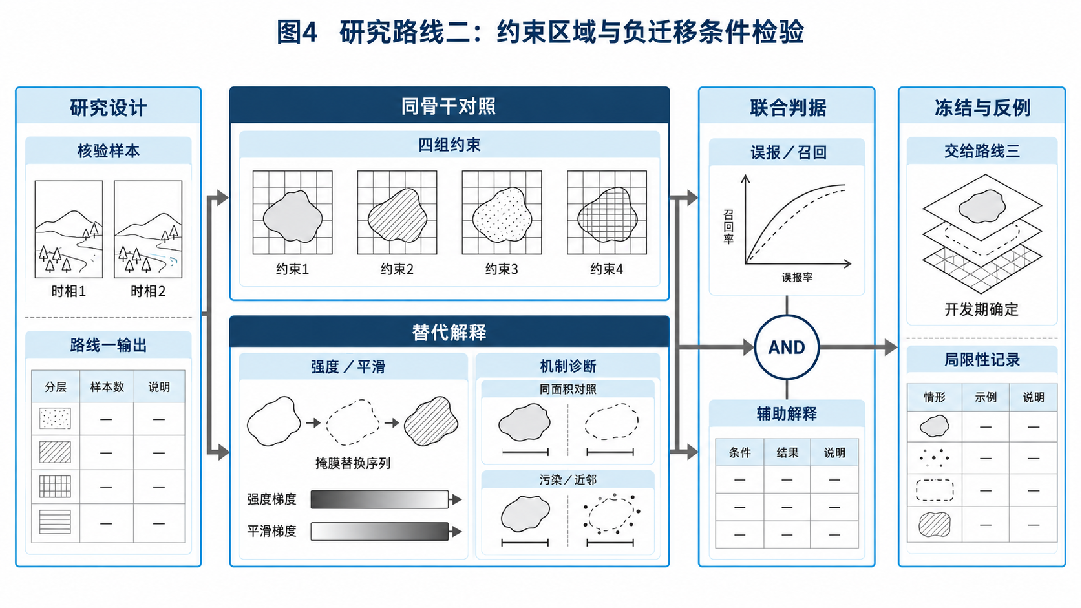
\includegraphics[width=\linewidth,trim=0 0 0 12mm,clip]{figures/F04_route_constraint.pdf}
  \captionsetup{justification=justified,singlelinecheck=false}
  \caption{研究路线二：约束区域与负迁移条件检验。四组依次为无一致性、全区域、背景位置与等面积随机约束；以误报改善和小变化召回非劣联合检验收益。曲线、掩码及表格均为研究设计示意，不是测量结果。}
  \label{fig:mct-route-constraint}
\end{figure}
\FloatBarrier

\textbf{（4）校准、错误排序与复核效用。}
在冻结模型后，利用独立校准矿区最小化概率对数损失拟合温度$T$；同时报告Brier分数、分组校准误差及类别分层可靠性曲线，防止背景占比主导结论。将整幅有效区域划为固定、不重叠窗口，预测未变化区同样进入候选集合。每个窗口根据概率熵、固定多视图预测分歧及其简洁加权组合排序；视图仅使用预先冻结且可逆对齐的变换，测试时不更新模型参数或归一化统计。窗口尺度、分数汇总和组合权重只依据验证矿区确定。

以每个矿区相同的有效面积比例分配复核预算，按顺序选取完整窗口，遇到首个会超预算的窗口即停止，累计面积不超过预算；边缘窗口按有效面积计费，记录实际复核比例和未用余额，所有排序方法采用相同规则。建议\textbf{【暂定 主复核预算为10\%有效面积，0、5\%、20\%及完整风险—覆盖率曲线为补充】}。分别比较随机、原始熵、校准熵、单独分歧与组合，随机排序重复后报告波动。不同窗口数量和有效面积不能混作同一预算。

为区分预算上限下的策略收益与排序本身的收益，增加等实际面积核对：在每一矿区取各排序实际选中面积的最小值作为共同面积，沿冻结的窗口序列及窗内行列顺序截取相同数量的有效像素，重新计算剩余错误。只有主预算和共同面积分析结论一致，才把改善归于排序。截取末窗仅用于像素面积意义上的离线敏感性分析，不当作实际整窗人工效率证据。

离线评估将被选中窗口内预测替换为真值，计算全图剩余FP及FN；相应比率仍以全图背景面积和全图变化面积为分母。选中区域中的真实变化覆盖、未选中区漏检与高置信度漏检另报。

主对照为验证集按预列规则选定的最强单指标排序，测试前固定。辅助假说只有在主预算下相对该对照的剩余FP和FN配对差的区间上界均小于零时，才称观察结果支持双降；仅点估计双降则称描述性改善，只改善一项则描述具体取舍。该结论保持辅助探索定位，不能无额外预注册即升级为与主假说并列的确认性发现。真值替换代表理想复核上限，真实复核还需记录核验者错误、耗时与一致性，不能用理想曲线宣称已节省人工工时。结论仅适用于所冻结的检测器及矿区范围；零基线错误矿区报告绝对差，不计算除零的相对改善。

\begin{figure}[!htbp]
  \centering
  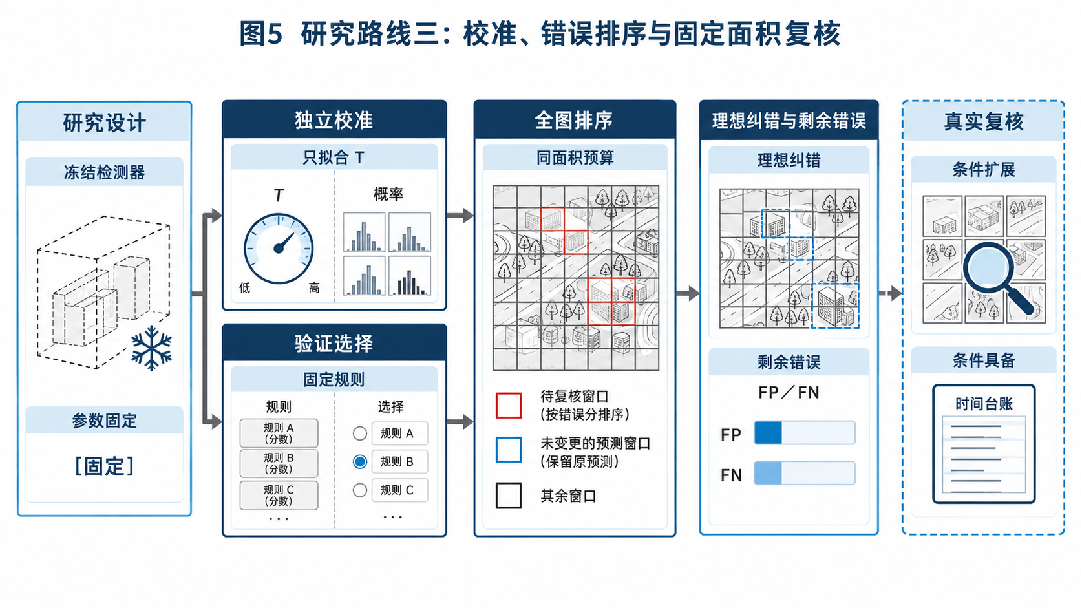
\includegraphics[width=\linewidth,trim=0 0 0 12mm,clip]{figures/F05_route_reliability.pdf}
  \captionsetup{justification=justified,singlelinecheck=false}
  \caption{研究路线三：校准、错误排序与固定面积复核。独立校准矿区只拟合温度，验证矿区选择排序规则；全图窗口进入候选集合。分布与窗口为示意，真值替换仅评价理想纠错上限，真实复核另需实施。}
  \label{fig:mct-route-reliability}
\end{figure}
\FloatBarrier

\textbf{（5）外部验证与矿山语义。}
核心实验完成后，视资源开展EuroMineNet内部矿区隔离验证，先建立其自身足迹变化基线，再明确年度足迹增减与主数据二值变化的对应关系。波段、分辨率和时相对齐后的迁移结果单列；若使用目标域信息则标明适应条件。全球铜矿静态边界仅用于名称、坐标和属性均能核对的案例匹配，样本不足时不作有色金属矿总体推断。专业解释由真实参与的合作者核验，未落实前只作影像与标签层面分析。标签连通域是制图单元，不直接对应独立采矿事件；实际判读若没有更可靠影像或现场证据，只报告判读一致性，不能认证真实采矿变化。

\subsubsection{关键技术}
一是建立矿区到原始场景和切片的来源映射，将模型选择、校准与最终测试分开，保证结论确实针对未见矿区。二是构建区域、面积、边界和强度均可追溯的一致性对照，使性能变化能够回到假说而非实现差异。三是把可靠性信息转化为整幅影像的复核顺序，联合核算误报、漏检、覆盖和工作量，识别校准有效但排序无增量的情况。这三项技术分别支撑数据可信、机制可检验和结果可解释。

\subsubsection{可行性分析}
公开数据具有正式发布入口，变化检测和域泛化存在可比近邻方法，允许从较小模型与固定骨干开展研究；当前可行性仍须以归档验收和基线运行检验。方法改动集中在训练约束与评测环节，不依赖从零训练大型基础模型。现有GPU与软件工具链支持启动单卡配置测量，再按实际可分配时段安排多种子实验；不将设备总数视为课题独占配额。

本课题的数据处理、模型训练和评测由申请人组织，拟参与人员为\textbf{【待补 F-MCT-01：实际成员、分工及投入时间】}，标签解释与矿山案例复核由\textbf{【待补 F-MCT-02：遥感或地质环境合作者及已落实安排】}承担。人员和合作落实后，将先验证工作量能否覆盖主数据、关键近邻与核心消融，再决定扩展实验。上述条件尚未齐备时，以单数据集、单机制及离线复核评价形成保守研究范围。
